\documentclass{./template/article}

\usepackage{booktabs}
\newcommand{\urwid}{\inlinetext{urwid}}
\newcommand{\yes}{\ding{52}}
\newcommand{\no}{\ding{56}}

% 设置标题和作者
\maintitle{\urwid{} 中文文档}
\authorname{张琦}
\abstract{
}

\begin{document}
\section{\urwid{} 概述}
\indent\urwid{} 是为 python 设计的控制台的 UI 库. \urwid{} 可以代替库 \inlinetext{curses} 来对控制台界面进行操作, 更加便捷, 简单.%
%
\begin{figure}[!htb]
    \centering
    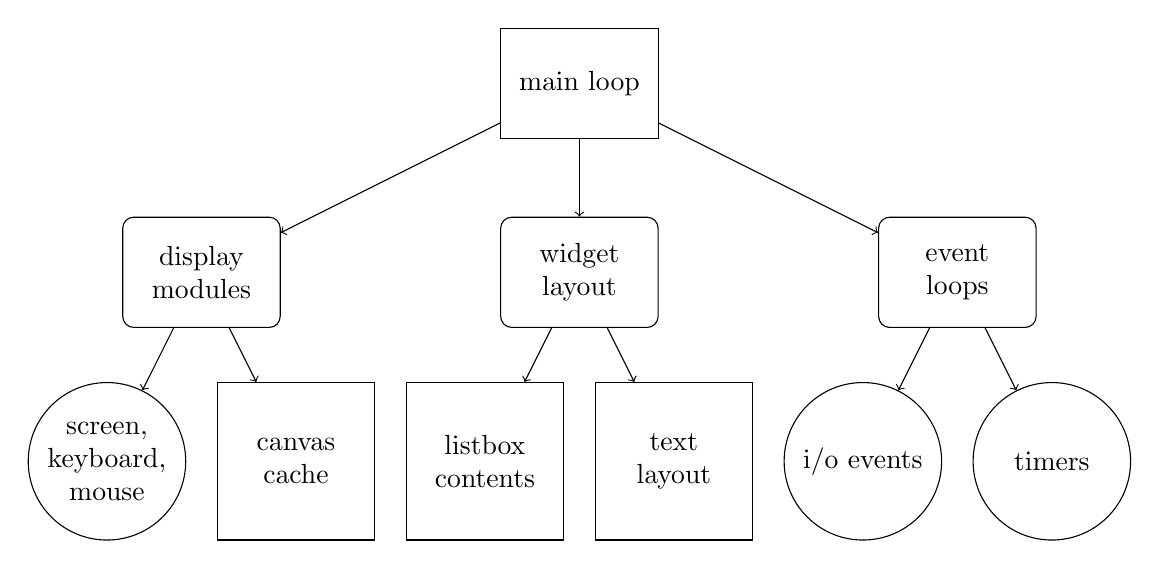
\begin{tikzpicture}[
  rectblock/.style = {rectangle, draw, inner sep = 0pt, align = flush center, minimum width = 2cm, minimum height = 1.4cm},
  roundblock/.style = {rectblock, rounded corners},
  circleblock/.style = {circle, draw, inner sep = 0pt, align = flush center, minimum size = 2cm},
  squareblock/.style = {rectblock, draw, align = flush center, inner sep = 0pt, minimum width = 2cm, minimum height = 2cm},
  x = 1.2cm,
  y = 0.8cm
]
  \node[rectblock]   (ml) at (7, 8) {main loop};
  \node[roundblock]  (dm) at (3, 5) {display\\modules};
  \node[roundblock]  (wl) at (7, 5) {widget\\layout};
  \node[roundblock]  (el) at (11, 5) {event\\loops};
  \node[circleblock] (skm) at (2, 2) {screen,\\keyboard,\\mouse}; 
  \node[squareblock] (cc) at (4, 2) {canvas\\cache};
  \node[squareblock] (lc) at (6, 2) {listbox\\contents};
  \node[squareblock] (tl) at (8, 2) {text\\layout};
  \node[circleblock] (io) at (10, 2) {i/o events};
  \node[circleblock] (ti) at (12, 2) {timers};
  
  \draw[->] (ml) -- (dm);
  \draw[->] (ml) -- (wl);
  \draw[->] (ml) -- (el);
  \draw[->] (dm) -- (cc);
  \draw[->] (dm) -- (skm);
  \draw[->] (wl) -- (lc);
  \draw[->] (wl) -- (tl);
  \draw[->] (el) -- (io);
  \draw[->] (el) -- (ti);
\end{tikzpicture}
    \caption{Caption}
    \label{fig:structure_of_urwid_library}
\end{figure}%
%
\urwid{} 的框架如\cref{fig:structure_of_urwid_library} 所示, 可见 \urwid{} 在设计之初, 就充分考虑了组件间解耦以及可扩展性.

显示模块 (display module) 负责接收用户输入, 然后将控制序列解释成键盘以及鼠标事件. 显示模块也可以用来绘制丰富的内容.

利用内置的组件可以很容易的搭建例子. 你应当把 \urwid{} 看成是一个控制台组件的集合, 而不是一个像 \inlinetext{GTK} 或是 \inlinetext{Qt} 一样的 UI 库. \urwid{} 提供的基础组件仅仅描述了它们如何在屏幕上排布.

在控制台界面中, 最多的组件就是文本 \inlinetext{Text}. \urwid{} 提供了大量的文本编码, 并且提供了一个可配置的文本布局, 可以满足大部分的对齐和断行需求. 如果你需要更加灵活的功能, 你也可以自己实现一个文本布局类.

\urwid{} 支持一些列通用显示功能, 其中包括 256 色前景色和背景色, 加粗, 下划线等等出色的显示配置. 值得注意的是, 这些功能有些终端软件并不支持, 因此, \urwid{} 可以帮助你实现一个可以自动检测终端类型并进行适配的软件.

列表框 \inlinetext{ListBox} 是 \urwid{} 中最强大的组件, 你可以用内置的遍历类也可以自己实现一个遍历类来控制列表框, 可以被用于实现列表框的滚动操作, 嵌套, 折叠以及一些类似的特性.

当组件被渲染到屏幕上的时候, 一个组件的弱引用会被保存在缓存中, 因此, 当这个组件被再次渲染的时候会特别的快. 由于是弱引用, \urwid{} 的显示模块将保持这个引用, 并用当前数据填充.

\urwid{} 的主循环简化了屏幕输入和更新的处理过程. 你也可以使用大量的事件循环, 并且支持集成 \inlinetext{Twisted} 的 Reactor 以及 \inlinetext{Glib} 的事件循环.
\section{主循环}
主循环 \inlinetext{MainLoop} 与显示模块, 组件集合以及时间循环是绑定的. \inlinetext{MainLoop} 负责将显示模块的输入传递给组件, 并渲染组件.

利用 \inlinepython{MainLoop.input_filter()} 方法, 你可以实现屏蔽用户输入的功能, 或者利用一些特殊的代码去拦截用户输入, 使用户输入无法达到组件, 比如 \inlinepython{MainLoop.unhandled_input()} 方法.

使用 \inlinepython{MainLoop.set_alarm_at()} 或 \inlinepython{MainLoop.set_alarm_in()} 方法, 你可以设置定时任务. 这两个方法在调用回调函数后可以自动的调用 \inlinepython{MainLoop.draw_screen()} 方法. 如果你想关闭定时任务, 可以使用 \inlinepython{MainLoop.remove_alarm()} 方法.

当主循环正在运行时, 只要触发了 \inlinepython{ExitMainLoop} 异常, 都会退出主循环, 并释放所有资源. 如果任何其他的异常出现在主循环中, 主循环将关闭显示模块, 然后再进入该异常的处理模块, 以避免终端状态的不正常. 我们在这里强烈建议使用 \inlinetext{MainLoop}, 如果 \inlinetext{MainLoop} 无法满足你的需求, 你可以自己实现一个主循环, \urwid{} 中的其他部分不依赖于 \inlinetext{MainLoop}.
\section{显示模块}
\indent\urwid{} 的显示模块提供了一个抽象层用于绘制屏幕以及读取用户输入. 你应该根据你的程序特点选择不同的显示模块.

\begin{figure}[!htb]
    \centering
    \begin{tikzpicture}[
  block/.style = {rectangle, draw, minimum width = 3cm, minimum height = 3cm, inner sep = 0pt, align = flush center}
]
  \node[block, fill = cyan, minimum height = 6cm] (rd) at (0, 6) {\mintinline{python}{raw_display}};
  \node[block, fill = cyan] (cd) at (3.4, 7.5) {\mintinline{python}{curses_display}};
  \node[block, fill = cyan] (wd) at (6.8, 7.5) {\mintinline{python}{web_display}};
  \node[block, fill = cyan, minimum height = 6cm] (hf) at (10.2, 6) {\mintinline{python}{html_fragment}};
  
  \node[block] (nl) at (3.4, 4.5) {\inlinetext{ncurses} library};
  \node[block] (ac) at (6.8, 4.5) {\inlinetext{apache} / \inlinetext{CGI}};
  \node[block, minimum width = 6.4cm] (ct) at (1.7, 1.5) {console or terminal};
  \node[block] (wb) at (6.8, 1.5) {web browser};
  \node[block] (ht) at (10.2, 1.5) {html file};
\end{tikzpicture}
    \caption{\urwid{} 库中的显示模块}
    \label{fig:display_models_of_urwid_library}
\end{figure}

通常情况下, 你需要为 \inlinepython{MainLoop} 的构造函数指定显示模块, 如\cref{code:specify_the_curses_display_for_main_loop} 所示.%
%
\begin{codebox}[
  caption = 为 \inlinepython{MainLoop} 指定显示模块 \inlinepython{urwid.curses_display.Screen()},
  label = code:specify_the_curses_display_for_main_loop
]
loop = MainLoop(widget, ..., screen = urwid.curses_display.Screen())
\end{codebox}%
%
如果不指定显示模块, \inlinepython{MainLoop} 会采用默认值 \inlinepython{urwid.raw_display.Screen()}, 如\cref{code:specify_the_raw_display_for_main_loop} 所示.%
%
\begin{codebox}[
  caption = 为 \inlinepython{MainLoop} 指定显示模块 \inlinepython{urwid.raw_display.Screen()},
  label = code:specify_the_raw_display_for_main_loop
]
# These are the same
loop = MainLoop(widget, ...)
loop = MainLoop(widget, ..., screen = urwid.raw_display.Screen())
\end{codebox}%

\subsection[raw\_display 与 curses\_display 显示模块]{\inlinepython{raw_display} 与 \inlinepython{curses_display} 显示模块}
\indent\urwid{} 有两个显示模块, 分别用于终端和控制台的显示. \inlinepython{raw_display.Screen} 模块是一个纯 python 的显示模块, 没有任何外部依赖. \inlinepython{raw_display.Screen} 可以直接处理终端中的控制序列, 也是 \inlinepython{MainLoop} 中的默认显示模块. \inlinepython{curses_display.Screen} 模块利用了操作系统提供的 \inlinetext{curses} 或 \inlinetext{ncurses} 库. \inlinepython{curses_display.Screen} 模块做了屏幕更新的优化, 并且用 termcap 优化用户终端.

当检测到用户的终端只支持黑白模时, \inlinetext{curses} 和 \inlinetext{ncurses} 库将会自动禁用彩色模式, 所以, 当用 \inlinepython{curses_display.Screen} 注册一个调色板时, 需要为黑白模式单独设置一套属性. \cref{tab:differences_between_the_two_modules} 总结了两种模式的区别.%
%
\begin{table}[!htb]
  \centering
  \caption{\inlinepython{raw_display} 与 \inlinepython{curses_display} 显示模块区别}
  \label{tab:differences_between_the_two_modules}
  \begin{tabu}{rcc}
  \tabucline[1pt]{-}
                        & \inlinepython{raw_display} & \inlinepython{curses_display}\\
  \hline
    优化 C 代码	        & \no  & \yes\\
    兼容所有终端	    & \no  & \yes\makebox[0pt][l]{\textsuperscript{1}}\\
    支持 UTF-8 编码	    & \yes & \yes\makebox[0pt][l]{\textsuperscript{2}}\\
    不用加粗高亮	    & \yes\makebox[0pt][l]{\textsuperscript{3}} & \no\\
    支持 88 色或 256 色 & \yes & \no\\
    支持鼠标拖拽	    & \yes & \no\\
    支持外部事件循环    & \yes & \no\\
  \tabucline[1pt]{-}
  \multicolumn{3}{l}{\footnotesize1. 需要 termcap 存在, 并且 TERM 环境变量配置正确}\\[-3pt]
  \multicolumn{3}{l}{\footnotesize2. 需要 python 与 \inlinetext{ncurses} 库关联}\\[-3pt]
  \multicolumn{3}{l}{\footnotesize3. 需要 使用 \inlinetext{xterm} 或 \inlinetext{gnome-terminal}}\\
  \end{tabu}
\end{table}

\subsection{其它显示模块}
\subsubsection[CGI Web 显示模块 web\_display]{CGI Web 显示模块 \inlinetext{web_display}}
\indent\inlinepython{urwid.web_display} 可以使你的程序像一个在 Apache 环境下的 CGI 脚本, 而不是运行在终端中. 这个显示模块还处在概念验证阶段, 目前还存在安全和响应性能的问题亟待解决, 所以不建议在生产环境中使用. 例子中的 \inlinetext{tour.py} 和 \inlinetext{calc.py} 使用的就是这种现实模式.

\subsubsection[Screenshot 显示模块 html\_fragment]{屏幕截图显示模块 \inlinetext{html_fragment}}
\indent\urwid{} 的界面可以被渲染成 HTML. 每当 \inlinepython{html_fragment.HtmlGenerator.draw_screen()} 被调用时, \inlinepython{html_fragment.HtmlGenerator} 显示模块可以通过模拟用户输入然后捕捉屏幕为 HTML 片段. 这些片段可能被包含在 HTML 文档中, 并且可以被浏览器正确渲染, 这需要使用等款字体, 并且需要标记为 \inlinetext{<pre>}. HTML 渲染出来的界面可以被搜索, 也可以被选中, 如果用户调整浏览器的字体, 这些文本也可以同步的进行缩放.

\subsubsection[LCD 显示模块 lcd\_display]{LCD 显示模块 \inlinetext{lcd_display}}
几乎所有的设备在网格中显示字符都可以被当做一个显示器. \inlinetext{lcd_display} 显示模块为 LCD 显示器的字符显示提供一些基类, 包 \inlinepython{lcd_display.CF635Screen} 就是为 Crystal Fontz 635 USB 这款设备设计的.

\subsection{设置调色板}
\indent\inlinetext{MainLoop} 的构造函数可以接受 \inlinepython{palette} 参数, 并且参数 \inlinepython{palette} 的值会被传递给显示模块的 \inlinepython{register_palette()} 方法. 调色板 \inlinepython{palette} 是一个显示属性名字以及前景色背景色设置构成的列表. 显示模块可能运行在黑白模式中, 正常模式或者高彩色模式, 你应该为每一个模式设置不同的前景色和背景色, 如\cref{code:example_of_palette} 所示.

\begin{codebox}[
  caption = 调色板举例,
  label = code:example_of_palette
]
palette = [
    ('headings', 'white,underline', 'black', 'bold,underline'), # bold text in monochrome mode
    ('body_text', 'dark cyan', 'light gray'),
    ('buttons', 'yellow', 'dark green', 'standout'),
    ('section_text', 'body_text'), # alias to body_text
]

loop = MainLoop(widget, palette = palette)
\end{codebox}

\section{组件}
\subsection{组件布局}
\indent\urwid{} 利用组件分割屏幕空间. 使得实现动态的界面十分容易, 可以适应不同的终端和字体大小. \cref{fig:example_of_widget_layout} 是一个 \urwid{} 布局的例子.%
%
\begin{figure}[!htb]
    \centering
    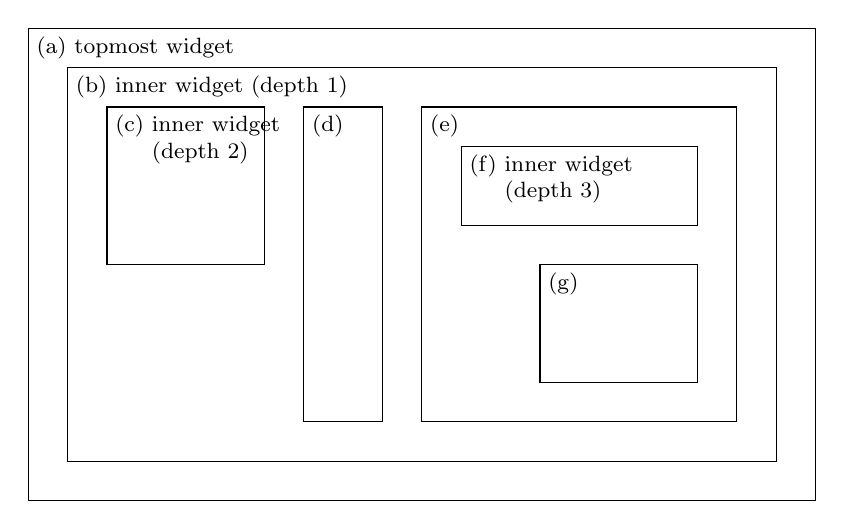
\begin{tikzpicture}[
  block/.style = {rectangle, draw},
  number/.style = {anchor = north west, inner sep = 3pt, font = \footnotesize, align = flush left}
]
  \node[block, minimum width = 10cm, minimum height = 6cm]   (a) at (5,   5.5)  {};
  \node[block, minimum width = 9cm,  minimum height = 5cm]   (b) at (5,   5.5)  {};
  \node[block, minimum width = 2cm,  minimum height = 2cm]   (c) at (2,   6.5)  {};
  \node[block, minimum width = 1cm,  minimum height = 4cm]   (d) at (4,   5.5)  {};
  \node[block, minimum width = 4cm,  minimum height = 4cm]   (e) at (7,   5.5)  {};
  \node[block, minimum width = 3cm,  minimum height = 1cm]   (f) at (7,   6.5)  {};
  \node[block, minimum width = 2cm,  minimum height = 1.5cm] (g) at (7.5, 4.75) {};
  
  \node[number] at (a.north west) {(a) topmost widget};
  \node[number] at (b.north west) {(b) inner widget (depth 1)};
  \node[number] at (c.north west) {(c) inner widget\\\hphantom{(c) }(depth 2)};
  \node[number] at (d.north west) {(d)};
  \node[number] at (e.north west) {(e)};
  \node[number] at (f.north west) {(f) inner widget\\\hphantom{(f) }(depth 3)};
  \node[number] at (g.north west) {(g)};
\end{tikzpicture}
    \caption{\urwid{} 布局举例}
    \label{fig:example_of_widget_layout}
\end{figure}%
%
组件的渲染会适应屏幕的大小, 当渲染最前面的组件时:%
%
\begin{itemize}
  \item 组件 (a) 全屏渲染.
  \item 在组件 (a) 上渲染组件 (b) 时, 是全屏渲染.
  \item 在组件 (b) 上渲染组件 (c), (d), (e) 时, 会将显示区域分割成三列.
  \item 在组件 (e) 上渲染最近 (f), (g) 时, 会将显示区域分割成两行.
  \item 组建 (e) 将组件 (f) 和 (g) 组合后一起返回.
  \item 组件 (b) 将组件 (c), (d) 和 (e) 组合后一起返回.
  \item 组件 (a) 与组件 (b) 组合, 并返回.
\end{itemize}%
%
组件 (a), (b) 和 (e) 被称为容器, 因为他们可以承载其它组件. 容器决定了其包含的组件的大小和位置. 容器必须跟踪当前的焦点组件. 在\cref{fig:example_of_widget_layout} 
中, 组件 (e) 的焦点组件是组件 (f), 同样, 组件 (e) 也是 (b) 的焦点组件. 如果组件 (f) 是一个文本框, 那么用户的输入将按照如下方式处理.%
%
\begin{itemize}
  \item 组件 (a) 将按键信息传给焦点组件 (b).
  \item 组件 (b) 将按键信息传给焦点组件 (e).
  \item 组件 (e) 将按键信息传给焦点组件 (f).
  \item 组件 (f) 要么处理按键, 要么直接返回这个按键信息.
  \item 如果组件 (f) 返回按键信息, 则组件 (e) 要么处理按键, 要么直接返回这个按键信息.
  \item 如果组件 (e) 返回按键信息, 则组件 (b) 要么处理按键, 要么直接返回这个按键信息.
  \item 如果组件 (b) 返回按键信息, 则组件 (a) 处理按键信息.
\end{itemize}

\subsection{盒子组件, 瀑布流组件和固定组件}
组件的尺寸的单位是屏幕的行数和列数. 行数和列数都给定的组件被称为盒子组件. 最上层的组件必须是盒子组件. 控制台中的大部分信息都是文本, 显示文本的最佳方式是瀑布流的形式, 承载这种显示内容的组件被称为瀑布流组件. 瀑布流组件需要指定列数, 而不用指定行数, 他可以根据需求自己计算行数. 有一种组件可以知道自己尺寸, 这种组件被称为固定组件. 这三种组件的尺寸计算如\cref{tab:how_a_widgets_size_is_determined} 所示.%
%
\begin{table}[!htb]
    \caption{三种组件尺寸计算}
    \label{tab:how_a_widgets_size_is_determined}
    \centering
    \begin{tabu}{lll}
    \tabucline[1pt]{-}
      组件类型 & 宽 & 长\\
    \hline
      盒子组件 & 由容器决定 & 由容器决定\\
      瀑布流组件 & 由容器决定 & 由组件的 \smash{\inlinepython{row()}} 方法决定 \\
      固定组件 & 由组件的 \smash{\inlinepython{pack()}} 方法决定 & 由组件的 \smash{\inlinepython{pack()}} 方法决定\\
    \tabucline[1pt]{-}
    \end{tabu}
\end{table}

\indent\urwid{} 有一个约定, 那就是用变量 \inlinepython{maxcol} 和 \inlinepython{maxrow} 存储组件的尺寸. 盒子组件需要同时指定变量 \inlinepython{maxcol} 和 \inlinepython{maxrow}. 瀑布流组件需要一个 \inlinepython{(maxcol,)} 来指定尺寸, 因为瀑布流的高度可以根据内容自动计算. 固定组件需要 \inlinepython{()} 来指定尺寸, 因为固定组件会自动计算自身尺寸.

\subsection{内建组件}
\indent\urwid{} 内建组件如\cref{fig:included_widgets} 所示.%
%
\begin{figure}[!htb]
    \centering
    \resizebox{\textwidth}{!}{\def\hsep{3.6cm}
\def\vsep{-0.2cm}

\definecolor{cflow}{rgb}{0.91, 0.78, 0.69}
\definecolor{cbox}{rgb}{0.69, 0.78, 0.91}
\definecolor{cfixed}{rgb}{1.00, 0.93, 0.67}

\begin{tikzpicture}[
  all/.style = {fill plain picture = {
    \draw[cfixed, line width = 2.5cm] (-1,-2) -- (3,2);
    \draw[cbox,   line width = 2.5cm] (-3,-2) -- (1,2);
    \draw[cflow,  line width = 1.2cm] (-2,-2) -- (2,2);
  }},
  box/.style = {fill = cbox},
  flow/.style = {fill = cflow},
  fixed/.style = {fill = cfixed},
  boxflow/.style = {fill plain picture = {
    \node[fill = cbox, line width = 0pt, draw = none, minimum size = 4cm, rotate = 45, anchor = south] at (0, 0) {};
    \node[fill = cflow, line width = 0pt, draw = none, minimum size = 4cm, rotate = 45, anchor = north]  at (0, 0) {};
  }},
  title/.style = {rectangle, minimum width = 3cm, minimum height = 0.5cm, text width = 3cm, align = left, font = \bfseries\ttfamily, inner sep = 0pt},
  widget/.style = {title, draw, font = \footnotesize\normalfont\ttfamily},
  blank/.style = {widget, minimum height = 2.4cm},
  shorten >= 0.2cm,
  shorten <= 0.2cm,
]
  \linespread{1}
  \node[title, flow] (text) {Text};
  \node[blank, anchor = north] (text') at ([yshift = \vsep]text.south) {text content wrapped or clipped to fill the available width, may also contain attributes (colors, underline, bold)\\\ };
  
  \node[title, flow] (edit) at ([xshift = \hsep]text) {Edit};
  \node[blank, anchor = north] (edit') at ([yshift = \vsep]edit.south) {user-editable text with an optional caption\\\ \\\ \\\ \\\ };
  
  \node[title, flow] (button) at ([xshift = \hsep]edit) {Buttons etc.};
  \node[blank, anchor = north, minimum height = 0.6cm] (button1) at ([yshift = \vsep]button.south) {  <Button>};
  \node[blank, minimum height = 0.6cm] (button2) at (edit' -| button) {  [ ] CheckBox};
  \node[blank, anchor = south, minimum height = 0.6cm] (button3) at (edit'.south -| button) {  ( ) RadioButton};
  
  \node[title, box] (solidfill) at ([xshift = \hsep]button) {SolidFill};
  \node[blank, anchor = north, align = flush center] (solidfill') at ([yshift = \vsep]solidfill.south) {xxxxxxxxxxxxxxxxxxxxx\\xxxxxxxxxxxxxxxxxxxxx\\xxxxxxxxxxxxxxxxxxxxx\\xxxxxxxxxxxxxxxxxxxxx\\xxxxxxxxxxxxxxxxxxxxx\\xxxxxxxxxxxxxxxxxxxxx\\xxxxxxxxxxxxxxxxxxxxx};
  
  \node[title, flow] (divider) at ([xshift = \hsep]solidfill) {Divider};
  \node[blank, anchor = north, align = flush center] (divider') at ([yshift = \vsep]divider.south) {};
  \draw ([yshift = 0.2cm]divider'.west) -- ([yshift = 0.2cm]divider'.east);
  \draw ([yshift = -0.2cm]divider'.west) -- ([yshift = -0.2cm]divider'.east);
  \draw[dashed] ([xshift = 0.5cm]divider'.west) -- ([xshift = -0.5cm]divider'.east);
  \draw[<->] (divider'.north) -- ([yshift = 0.2cm]divider'.center);
  \draw[<->] (divider'.south) -- ([yshift = -0.2cm]divider'.center);

  \node[title, box] (bargraph) at ([yshift = -5cm]text) {BarGraph};
  \node[blank, anchor = north, align = flush center] (bargraph') at ([yshift = \vsep]bargraph.south) {%
    \begin{minipage}[t]{3cm}
\begin{verbatim}
    xx   xx          
   xxx   xxx xxx     
   xxx   xxx xxx     
   xxx   xxx xxxxxxxx
xx xxx   xxx xxxxxxxx
xx xxxxxxxxx xxxxxxxx
xxxxxxxxxxxxxxxxxxxxx
\end{verbatim}
    \end{minipage}
  };
  
  \node[title, box] (graphvscale) at ([xshift = \hsep]bargraph) {GraphVScale};
  \node[blank, anchor = north, align = flush left] (graphvscale') at ([yshift = \vsep]graphvscale.south) ;
  
  \node[title, fixed] (bigtext) at ([xshift = \hsep]progressbar) {BigText};
  \node[blank, anchor = north, align = flush center] (bigtext') at ([yshift = \vsep]bigtext.south) {%
  \begin{minipage}[t]{3cm}
\begin{verbatim}
        x            
 xxxx   x            
     x  x            
 xxxxx  xxxxx    xxxx
x    x  x    x  x    
x    x  x    x  x    
 xxxxx  xxxxx    xxxx
\end{verbatim}
  \end{minipage}
  };
  
  \node[all, title] (padding) at ([yshift = -5cm]bargraph) {Padding};
  \node[blank, anchor = north, align = flush center] (padding') at ([yshift = \vsep]padding.south) {};
  \node[blank, all, minimum width = 1.5cm, text width = 1.5cm, align = flush center] (padding'') at (padding') {\texttt{original\_}\\\texttt{widget}};
  \draw[<->] (padding'.west) -- (padding''.west);
  \draw[<->] (padding'.east) -- (padding''.east);
  
  
  \node[box, title] (filler) at ([xshift = \hsep]padding) {Filler};
  \node[blank, anchor = north, align = flush center] (filler') at ([yshift = \vsep]filler.south) {};
  \node[blank, boxflow, minimum height = 0.6cm, align = flush center] (filler'') at (filler') {\texttt{original\_}\\\texttt{widget}};
  \draw[<->] (filler'.north) -- (filler''.north);
  \draw[<->] (filler'.south) -- (filler''.south);
  
  \node[all, title] (attrmap) at ([xshift = \hsep]filler) {AttrMap};
  \node[blank, all, anchor = north, align = flush center] (attrmap') at ([yshift = \vsep]attrmap.south) {original\_widget (with attributes possibly altered)};
  
  \node[flow, title] (boxadapter) at ([xshift = \hsep]attrmap) {BoxAdapter};
  \node[blank, box, anchor = north, align = flush center] (boxadapter') at ([yshift = \vsep]boxadapter.south) {original\_widget};
  
  \node[boxflow, title] (linebox) at ([xshift = \hsep]boxadapter) {LineBox};
  \node[blank, anchor = north] (linebox') at ([yshift = \vsep]linebox.south) {};
  \node[blank, dashed, minimum height = 2cm, minimum width = 2.6cm, text width = 0cm, inner sep = 0pt] at (linebox') {};
  \node[blank, boxflow, align = flush center, minimum width = 2.2cm, minimum height = 1.6cm, text width = 2.2cm] at (linebox') {original\_widget};
  
  
  \node[boxflow, title] (columns) at ([yshift = -5cm]padding) {Columns};
  \node[blank, boxflow, anchor = north, align = flush center, minimum width = 1.2cm, text width = 1cm] (columns') at ([yshift = \vsep, xshift = -0.9cm]columns.south) {widget\_\\list[0]};
  \node[blank, boxflow, anchor = north, align = flush center, minimum width = 1.2cm, text width = 1cm] (columns') at ([yshift = \vsep, xshift = 0.3cm]columns.south) {widget\_\\list[1]};
  \node[blank, boxflow, anchor = north, align = flush center, minimum width = 0.6cm, text width = 1cm, text width = 0.6cm] (columns') at ([yshift = \vsep, xshift = 1.2cm]columns.south) {...};
\end{tikzpicture}}
    \caption{\urwid{} 内建组件}
    \label{fig:included_widgets}
\end{figure}%
%
基本组件和图形组件用来和用户进行交互, 也可以成为自定义组件的一部分. 除此之外还有修饰组件和容器组件, 下面分别对修饰组件和容器组件进行详细介绍.

\subsection{修饰组件}
修饰组件可以更改单个组件的外观和位置. 可以访问修饰组件的 \inlinepython{original_widget} 属性访问其所包含的组件. 如果你使用多个装饰组件, 则可以通过 \inlinepython{base_widget} 来访问 \inlinepython{original_widget}. \inlinepython{Widget.base_widget} 指向所有非修饰组件的 \inlinepython{self} 变量, 所以修饰组件在任何条件下都是安全的.

\subsection{容器组件}
容器组件可以将自身的可用空间按照其所包含的组件分割成若干部分, 即组件的布局. 在处理可选中的组件时, 容器组件同时可以跟踪其子组件的焦点. 容器组件可以互相嵌套, 因此, 焦点所在的组件可能比最上面的组件低跟多层. 不论你使用何种类型的容器组件, 你都可以使用 \urwid{} 提供的通用 API. 对于访问和修改内容的特定的旧方法, 仍然保持向后兼容性, 但是, 这个 API 现在是修改和遍历容器的首选方法.

\indent\inlinepython{container.focus} 是一个只读属性, 可以返回该容器中焦点所在的组件. 如果容器组件是空的, 或者是非容器组件, 那么将返回 \inlinepython{None}.

\indent\inlinepython{container.focus_position} 是一个可读写的属性, 可以用来访问容器中焦点空间的位置. 这通常是一个整数值, 但也可以是任何对象. 使用\inlinepython{SimpleListWalker} 或 \inlinepython{SimpleFocusListWalker} 作为其主体的 \inlinepython{Columns}, \inlinepython{Pile}, \inlinepython{GridFlow}, \inlinepython{Overlay} 和 \inlinepython{ListBox} 是使用整数作为其位置参数. 而 \inlinepython{Frame} 使用 \inlinepython{body}, \inlinepython{header} 和 \inlinepython{footer} 作为其位置参数. 带有自定义列表遍历器的 \inlinepython{ListBox} 将使用列表遍历器返回值作为位置参数. 如果访问一个空容器或者一个非容器组件的 \inlinepython{focus_position} 参数, 会引发 \inlinepython{IndexError} 异常. 对这个属性进行非法赋值, 也会引发 \inlinepython{IndexError} 异常. 对 \inlinepython{focus_position} 赋值, 将会自动将该组件标记为需要重绘.

\indent\inlinepython{container.contents} 是一个只读属性, 可以用来访问一个字典或者列表形式的子组件, 这些选项用来在此容器中显示这些子组件. 字典或者列表对象允许使用 \inlinepython{__getitem__()} 读取其元素, 并且支持通过调用 \inlinepython{__setitem__()} 和 \inlinepython{__delitem__()} 方法来进行赋值和删除. 当这个属性被修改, 该对象中的所有组件都将被标记为需要重绘. \inlinepython{Columns}, \inlinepython{Pile} 和 \inlinepython{GridFlow} 允许给其 \inlinepython{container.contents} 赋给一个新的迭代器, 来替换原来的值. \inlinepython{Columns}, \inlinepython{Pile}, \inlinepython{Overlay}, \inlinepython{GridFlow} 和 \inlinepython{Frame} 都支持 \inlinepython{container.contents} 元素的赋值和删除.

\indent\inlinepython{container.options(...)} 是一个成员方法, 可以返回用于添加到容器中的可选对象. 参数列表是容器类型, 与容器的构造函数 \inlinepython{__init__()} 的参数基本一致. 该方法返回的对象是一个由字符串和整数构成的元组, 如果容器没有子组件选项, 则返回 \inlinepython{None}. 这个方法的存在, 使得 \urwid{} 将来的版本也可以向已有的容器添加新的选项. 当添加新选项时, 期望选项元组保持不变的代码都将失败, 因此, 强烈建议使用选项元组进行防御性编程.

\indent\inlinepython{container.__getitem__(x)}, 该方法可以被简写成 \inlinepython{container[x]}, 是一个快捷方法, 其作用于 \inlinepython{container.contents[x][0].base_widget} 的作用相同. 其作用是返回位置在 \inlinepython{x} 的子组件, 并且忽略所有的修饰组件. 修饰组件包含 \inlinepython{Padding}, \inlinepython{Filler}, \inlinepython{AttrMap} 等等.
% \clearpage
% \phantomsection
% \addcontentsline{toc}{section}{参考文献}
% \bibliographystyle{ieeetr}
% \bibliography{./references}
\end{document}
